\todo{Biharmonic Operator instead of Bi-laplace!}\todo{Make clear that we consider PDE operators that consist of sums}Using neural networks to learn functions constrained by physical laws is a popular trend in scientific machine learning \cite{carleo2017solving, pfau2020ab, hermann2020deep, karniadakis2021physics, raissi2019physics, hu2023hutchinson, sun2020global}.
Typically, the physics is encoded through partial differential equations (PDEs) that the neural net must satisfy.
The associated loss functions require evaluating differential operators \wrt the network's input, rather than weights.
Evaluating differential operators remains a computational challenge, especially if they contain high-order derivatives.

\paragraph{Computing PDE operators.} Two important fields that require the evaluation of PDE operators are variational Monte-Carlo (VMC) simulations and physics-informed neural networks (PINNs).
VMC employs neural networks as an ansatz for the Schr\"odinger equation \cite{carleo2017solving, pfau2020ab, hermann2020deep} and demands computing the net's Laplacian, i.e., the Hessian trace usually in a non-differentiable fashion.
PINNs represent PDE solutions as a neural network and train the network via minimizing the residuals of the governing equations \cite{raissi2019physics, karniadakis2021physics}. For instance, Kolmogorov-type equations—including the Fokker-Planck and Black-Scholes equation—requires the differentiable evaluation of weighted second-order derivatives on high-dimensional spatial domains \cite{hu2023hutchinson, sun2024dynamical}. For PINN applications in elasticity, the Biharmonic operator \cite{vahab_physics-informed_2022} requires the computation of fourth-order derivatives, making it a commonly considered a benchmarking problem for computing high-order derivatives in PINNs \cite{hu2023hutchinson, vikas_biharm, shi2024stochastic}.

\paragraph{Is backpropagation all we need?}
% Alternative: The gap between theory and practice
Although nesting first-order automatic differentiation (AD) to compute high-order derivatives scales poorly, this approach is common practice.
\todo{Felix, M: still needs citation.}
A promising alternative to nested backpropagation, especially for higher-order derivatives is \emph{Taylor-mode AD}~\cite[or simply \emph{Taylor-mode},][\S13]{griewank2008evaluating}, introduced to the machine learning community in \citeyear{bettencourt2019taylor} and the JAX ecosystem in \cite{bradbury2018jax}.
However, we observe empirically that vanilla Taylor-mode is often not enough to improve upon nested backpropagation: Evaluating the Laplacian of a 5-layer $\tanh$ activated MLP using JAX' \emph{Taylor mode is 50\% slower} than nested backpropagation via computing, then tracing, the Hessian via Hessian-vector products \cite{pearlmutter1994fast,dagreou2024how}. This calls into question the relevance of Taylor mode for computing common PDE operators.

\paragraph{Improved Taylor mode schemes}
However, recent works have successfully demonstrated the potential of modified forward propagation schemes.
For the (weighted) Laplacian, \citet{li2023forward, li2024dof} developed a special forward propagation framework called the \emph{forward Laplacian}.
Relating to our example above, JAX' forward Laplacian \cite{gao2023folx} is roughly twice as fast as nested backpropagation at reduced memory costs.
While the forward Laplacian does not rely on Taylor mode, recent work pointed out a connection \cite{dangel2024kroneckerfactored}; however, it remains unclear if efficient forward schemes can be derived for other differential operators. Another line of work concerns the stochastic approximation of differential operators in high-dimensions \citet{shi2024stochastic}, relying on Taylor mode with suitably sampled random directions. In this work we identify a mechanism to rewrite the computational graph of standard Taylor mode, applicable to general PDE operators and stochastic Taylor mode: Precisely, our contributions are:
\todo{Felix: Make it more explicit that we evaluate Taylor mode in multiple directions and then sum the results. The sum can be pulled inside.}

\begin{figure*}[!t]
  \centering
  \begin{minipage}[b]{0.42\linewidth}
    \centering
    \input{figures/vanilla_taylor_not_enough.tex}

    \caption{\textbf{$\blacktriangle$ Vanilla Taylor mode is not enough to beat nested 1\textsuperscript{st}-order AD.}
      Illustrated for computing the Laplacian of a $\mathrm{tanh}$-activated $50 \!\to\! 768 \!\to\! 768 \!\to\! 512 \!\to\! 512 \!\to\! 1$
      MLP with JAX (+ \texttt{jit}) on GPU (details in \Cref{sec:jax-benchmark}).
      We show how to automatically obtain the specialized forward Laplacian through simple graph transformations of vanilla Taylor mode.
    }\label{fig:vanilla-taylor-not-enough}

    \vspace{0.25ex}
    \caption{\textbf{$\blacktriangleright$ Our collapsed Taylor mode directly propagates the sum of highest degree coefficients.}
      Visualized for propagating four $K$-jets through a $\sR^5 \!\to\! \sR^3 \!\to\! \sR$ function ($K=2$ yields the forward Laplacian).
      \Cref{sec:background} introduces the notation.}\label{fig:visual-abstract}
  \end{minipage}
  \hfill
  \begin{minipage}[b]{0.57\linewidth}
    \centering
    \newcommand{\drawgridrectangle}[4]{%
  \begin{tikzpicture}[scale=#4]
    \pgfmathsetmacro{\ymax}{#1}
    \pgfmathsetmacro{\xmax}{#2}

    % Fill the rectangle
    \fill[#3] (0,0) rectangle (\xmax,\ymax);

    % Draw the border
    \draw[white, line width=#4*3pt] (0,0) rectangle (\xmax,\ymax);


    % Draw vertical grid lines
    \pgfmathsetmacro{\xsteps}{#2}
    \foreach \x in {1,...,\xsteps} {
      \draw[white, line width=#4*3pt] (\x,0) -- (\x,\ymax);
    }

    % Draw horizontal grid lines
    \pgfmathsetmacro{\ysteps}{#1}
    \foreach \y in {1,...,\ysteps} {
      \draw[white, line width=#4*3pt] (0,\y) -- (\xmax,\y);
    }
  \end{tikzpicture}%
}

\newsavebox{\taylorStandard}
\savebox{\taylorStandard}{
  \begin{tikzpicture}
    \matrix [%
    matrix of nodes,%
    ampersand replacement=\&,% to use inside a savebox
    nodes={anchor=center, align=center},%
    column sep=4ex,%
    row sep=1ex,%
    ] (taylor)
    {
      \drawgridrectangle{1}{3}{blue!30}{0.33} \& \drawgridrectangle{1}{2}{blue!30}{0.33} \& \drawgridrectangle{1}{1}{blue!30}{0.33}
      \\[-1.5ex]
      $\vx_0$ \& $\vh_0$ \& $\vg_0$
      \\
      \drawgridrectangle{3}{3}{green!30}{0.33} \& \drawgridrectangle{3}{2}{green!30}{0.33} \& \drawgridrectangle{3}{3}{green!30}{0.33}
      \\[-1.5ex]
      $\{\vx_{1,d}\}$ \& $\{\vh_{1,d}\}$ \& $\{\vg_{1,d}\}$
      \\
      \drawgridrectangle{3}{3}{red!30}{0.33} \& \drawgridrectangle{3}{2}{red!30}{0.33} \& \drawgridrectangle{3}{1}{red!30}{0.33} \& \drawgridrectangle{1}{1}{red!60}{0.33}
      \\[-1.5ex]
      $\{\vx_{2,d}\}$ \& $\{\vh_{2,d}\}$ \& $\{\vg_{2,d}\}$ \& $\sum_d \vg_{2,d}$
      \\
    };

    % draw dependencies
    \pgfmathsetmacro{\K}{3}
    \pgfmathsetmacro{\L}{2}

    \foreach \l in {1,...,\L}{
      \pgfmathsetmacro{\lother}{int(\l+1)}
      \foreach \k in {1,...,\K} {
        \pgfmathsetmacro{\row}{int(2*\k-1)}
        \foreach \kother in {\k,...,\K} {
          \pgfmathsetmacro{\rowother}{int(2*\kother-1)}
          \draw[-Stealth, line width=1pt, white!50!black] (taylor-\row-\l.east) -- (taylor-\rowother-\lother.west);
        }
      }
    }
    \pgfmathsetmacro{\Lstart}{int(\L + 1)}
    \pgfmathsetmacro{\Lend}{int(\L + 2)}
    \pgfmathsetmacro{\rowfinal}{int(2*\K - 1)}
    \draw[-Stealth, line width=1pt, white!50!black] (taylor-\rowfinal-\Lstart.east) -- (taylor-\rowfinal-\Lend.west);
  \end{tikzpicture}
}

\newsavebox{\taylorCollapsed}
\savebox{\taylorCollapsed}{
  \begin{tikzpicture}
    \matrix [%
    matrix of nodes,%
    ampersand replacement=\&,% to use inside a savebox
    nodes={anchor=center, align=center},%
    column sep=4ex,%
    row sep=1ex,%
    ] (taylor)
    {
      \drawgridrectangle{1}{3}{blue!30}{0.33} \& \drawgridrectangle{1}{2}{blue!30}{0.33} \& \drawgridrectangle{1}{1}{blue!30}{0.33}
      \\[-1.5ex]
      $\vx_0$ \& $\vh_0$ \& $\vg_0$
      \\
      \drawgridrectangle{3}{3}{green!30}{0.33} \& \drawgridrectangle{3}{2}{green!30}{0.33} \& \drawgridrectangle{3}{3}{green!30}{0.33}
      \\[-1.5ex]
      $\{\vx_{1,d}\}$ \& $\{\vh_{1,d}\}$ \& $\{\vg_{1,d}\}$
      \\[2ex]
      \drawgridrectangle{1}{3}{red!60}{0.33} \& \drawgridrectangle{1}{2}{red!60}{0.33} \& \drawgridrectangle{1}{1}{red!60}{0.33}
      \\[-1.5ex]
      $\sum_d \vx_{2,d}$ \& $\sum_d \vh_{2,d}$ \& $\sum_d \vg_{2,d}$
      \\[1.1ex]
      \& \&
      \\
    };

    % draw dependencies
    \pgfmathsetmacro{\K}{3}
    \pgfmathsetmacro{\L}{2}

    \foreach \l in {1,...,\L}{
      \pgfmathsetmacro{\lother}{int(\l+1)}
      \foreach \k in {1,...,\K} {
        \pgfmathsetmacro{\row}{int(2*\k-1)}
        \foreach \kother in {\k,...,\K} {
          \pgfmathsetmacro{\rowother}{int(2*\kother-1)}
          \draw[-Stealth, line width=1pt, white!50!black] (taylor-\row-\l.east) -- (taylor-\rowother-\lother.west);
        }
      }
    }
  \end{tikzpicture}
}

\begin{figure*}[!t]
  \centering
  \resizebox{\linewidth}{!}{%
    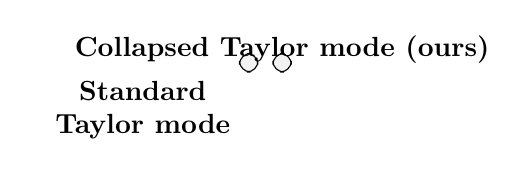
\begin{tikzpicture}
      \node (standard) [fill=black!5!white, draw=black, rounded corners]{\usebox{\taylorStandard}};
      \node [anchor=north east, align=center, inner sep=10pt] at (standard.north east) {\textbf{Standard} \\ \textbf{Taylor mode}};
      \node (collapsed) [fill=black!5!white, draw=black, rounded corners, anchor=north west, xshift=5pt] at (standard.north east) {\usebox{\taylorCollapsed}};
      \node [anchor=south, align=center, inner sep=3pt] at (collapsed.south) {\textbf{Collapsed Taylor mode (ours)}};
    \end{tikzpicture}
  }
  \caption{\textbf{Visual comparison of standard Taylor mode and our proposed collapsed Taylor mode.}}\label{fig:comparison-standard-vs-collapsed}
\end{figure*}

\begin{figure*}
  \centering
  \newsavebox{\taylorStandardNew}
  \savebox{\taylorStandardNew}{
    \begin{tikzpicture}
      \matrix [%
      matrix of nodes,%
      ampersand replacement=\&,% to use inside a savebox
      nodes={anchor=center, align=center},%
      column sep=5ex,%
      row sep=1ex,%
      ] (taylor)
      {
        \drawgridrectangle{1}{5}{gray!25!white}{0.33}
        \& \drawgridrectangle{1}{3}{gray!25!white}{0.33}
        \& \drawgridrectangle{1}{1}{gray!25!white}{0.33}
        \\[-1.5ex]
        $\vx_0$ \& $\vh_0$ \& $\vg_0$
        \\
        \drawgridrectangle{4}{5}{gray!50!white}{0.33}
        \& \drawgridrectangle{4}{3}{gray!50!white}{0.33}
        \& \drawgridrectangle{4}{1}{gray!50!white}{0.33}
        \\[-1.5ex]
        $\{\vx_{1,d}\}$ \& $\{\vh_{1,d}\}$ \& $\{\vg_{1,d}\}$
        \\[0.5ex]
        \drawgridrectangle{1}{5}{white}{0.33}
        \& \drawgridrectangle{1}{3}{white}{0.33}
        \& \drawgridrectangle{1}{1}{white}{0.33}
        \\[0.5ex]
        \\
        \drawgridrectangle{4}{5}{gray}{0.33}
        \& \drawgridrectangle{4}{3}{gray}{0.33}
        \& \drawgridrectangle{4}{1}{gray}{0.33}
        \\[-1.5ex]
        $\{\vx_{K-1,d}\}$ \& $\{\vh_{K-1,d}\}$ \& $\{\vg_{K-1,d}\}$
        \\[0.5ex]
        \drawgridrectangle{4}{5}{red!50}{0.33}
        \&
        \drawgridrectangle{4}{3}{red!50}{0.33}
        \&
        \drawgridrectangle{4}{1}{red!50}{0.33}
        \\[-1.5ex]
        $\{\vx_{K,d}\}$ \& $\{\vh_{K,d}\}$ \& $\{\vg_{K,d}\}$
        \\[-1.5ex]
        \textcolor{purple!50!red}{$\sum_d \vx_{K,d}$}
        \& \textcolor{purple!50!red}{$\sum_d \vh_{K,d}$}
        \& \textcolor{purple!50!red}{$\sum_d \vg_{K,d}$}
        \\
      };

      \node[xshift=-1pt, yshift=-14pt] at (taylor-9-1) {\drawgridrectangle{1}{5}{purple!50!red}{0.33}};
      \node[xshift=-1pt, yshift=-14pt] at (taylor-9-2) {\drawgridrectangle{1}{3}{purple!50!red}{0.33}};
      \node[xshift=-1pt, yshift=-14pt] at (taylor-9-3) {\drawgridrectangle{1}{1}{purple!50!red}{0.33}};

      \node at (taylor-5-1) {\vdots};
      \node at (taylor-5-2) {\vdots};
      \node at (taylor-5-3) {\vdots};

      % draw dependencies
      \pgfmathsetmacro{\K}{5}
      \pgfmathsetmacro{\L}{2}

      \foreach \l in {1,...,\L}{
        \pgfmathsetmacro{\lother}{int(\l+1)}
        \foreach \k in {1,...,\K} {
          \pgfmathsetmacro{\row}{int(2*\k-1)}
          \foreach \kother in {\k,...,\K} {
            \pgfmathsetmacro{\rowother}{int(2*\kother-1)}
            \draw[-Stealth, line width=1pt, gray] (taylor-\row-\l.east) -- (taylor-\rowother-\lother.west);
          }
        }
      }

      \coordinate (arrowStart) at ($(taylor-1-1.north)+(0,3.5ex)$);
      \coordinate (arrowEnd) at ($(taylor-1-3.north east)+(0,3.5ex)$);
      \draw[-Stealth, line width=2pt, black] (arrowStart) to node [midway, fill=white, align=center] {\textbf{Taylor forward} \\ \textbf{propagation}} (arrowEnd);

      \node [left=1.5ex of taylor-1-1] (zero) {0};
      \node [left=1.5ex of taylor-3-1] {1};
      \node [left=1.5ex of taylor-5-1] {$\vdots$};
      \node [left=1.5ex of taylor-7-1] {$K-1$};
      \node [left=1.5ex of taylor-9-1] {$K$};

      \node [align=center] (coefficientLabel) at ($(zero)+(0, 5.5ex)$) {\textbf{Derivative}\\\textbf{degree}};

      \draw[rounded corners] (taylor-9-1.north west) rectangle (taylor.south east);
    \end{tikzpicture}
  }

  \begin{tikzpicture}
    \node {\usebox{\taylorStandardNew}};
  \end{tikzpicture}
\end{figure*}

%%% Local Variables:
%%% mode: LaTeX
%%% TeX-master: "../main"
%%% End:

  \end{minipage}
\end{figure*}

\begin{enumerate}[leftmargin=0.5cm]
\item \textbf{We propose optimizing standard Taylor mode by collapsing the highest Taylor coefficients} by directly propagating their sum, rather than propagating then summing (\cref{fig:visual-abstract}). This recovers the forward Laplacian and is applicable to randomized Taylor mode. Furthermore, relying on a result of Griewank et al.\, \cite{griewank_evaluating_1999}, we show how to transform general PDE operators into a form amenable to our setting.

%and, relying on [...] can be generalized to 

  %Collapsing standard Taylor mode for the Laplacian yields the forward Laplacian \cite{li2023forward}, but we show that this optimization is applicable to many other differential operators, and stochastic Taylor mode \cite{shi2024stochastic}.
  \todo{Felix: Phrase this so that it becomes clear that this is a theoretical contribution.}

\item \textbf{We show how to collapse standard Taylor mode by simple graph rewrites based on linearity.}
  This leads to a clean separation of concepts:
  Users can build their computational graph using standard Taylor mode, then use graph rewrites to collapse it.
  Due to the simple nature of our proposed rewrites, this feature could easily be absorbed into the just-in-time (JIT) compilation of ML frameworks, without introducing a new interface.

\item \textbf{We empirically demonstrate the performance improvements of collapsed Taylor mode.} We introduce a Taylor mode library for PyTorch \cite{paszke2019pytorch} that realizes the graph simplifications with \texttt{torch.fx} \cite{reed2022torch}. Furthemore, we show that collapsing Taylor mode yields the theoretically expected improvements in run time and memory consumption. Due to the simple nature of our proposed rewrites, this feature could easily be integrated into the just-in-time (JIT) compilation of ML frameworks, without introducing a new interface.

\end{enumerate}

Our work takes an important step towards the broader adoption of Taylor mode as viable alternative to backpropagation for computing PDE operators, while being as easy to use. 

%%% Local Variables:
%%% mode: LaTeX
%%% TeX-master: "../main"
%%% End:
